% Options for packages loaded elsewhere
\PassOptionsToPackage{unicode}{hyperref}
\PassOptionsToPackage{hyphens}{url}
%
\documentclass[
]{article}
\usepackage{lmodern}
\usepackage{amssymb,amsmath}
\usepackage{ifxetex,ifluatex}
\ifnum 0\ifxetex 1\fi\ifluatex 1\fi=0 % if pdftex
  \usepackage[T1]{fontenc}
  \usepackage[utf8]{inputenc}
  \usepackage{textcomp} % provide euro and other symbols
\else % if luatex or xetex
  \usepackage{unicode-math}
  \defaultfontfeatures{Scale=MatchLowercase}
  \defaultfontfeatures[\rmfamily]{Ligatures=TeX,Scale=1}
\fi
% Use upquote if available, for straight quotes in verbatim environments
\IfFileExists{upquote.sty}{\usepackage{upquote}}{}
\IfFileExists{microtype.sty}{% use microtype if available
  \usepackage[]{microtype}
  \UseMicrotypeSet[protrusion]{basicmath} % disable protrusion for tt fonts
}{}
\makeatletter
\@ifundefined{KOMAClassName}{% if non-KOMA class
  \IfFileExists{parskip.sty}{%
    \usepackage{parskip}
  }{% else
    \setlength{\parindent}{0pt}
    \setlength{\parskip}{6pt plus 2pt minus 1pt}}
}{% if KOMA class
  \KOMAoptions{parskip=half}}
\makeatother
\usepackage{xcolor}
\IfFileExists{xurl.sty}{\usepackage{xurl}}{} % add URL line breaks if available
\IfFileExists{bookmark.sty}{\usepackage{bookmark}}{\usepackage{hyperref}}
\hypersetup{
  pdftitle={Markov Sick-Sicker model in R},
  pdfauthor={The DARTH workgroup},
  hidelinks,
  pdfcreator={LaTeX via pandoc}}
\urlstyle{same} % disable monospaced font for URLs
\usepackage[margin=1in]{geometry}
\usepackage{color}
\usepackage{fancyvrb}
\newcommand{\VerbBar}{|}
\newcommand{\VERB}{\Verb[commandchars=\\\{\}]}
\DefineVerbatimEnvironment{Highlighting}{Verbatim}{commandchars=\\\{\}}
% Add ',fontsize=\small' for more characters per line
\usepackage{framed}
\definecolor{shadecolor}{RGB}{248,248,248}
\newenvironment{Shaded}{\begin{snugshade}}{\end{snugshade}}
\newcommand{\AlertTok}[1]{\textcolor[rgb]{0.94,0.16,0.16}{#1}}
\newcommand{\AnnotationTok}[1]{\textcolor[rgb]{0.56,0.35,0.01}{\textbf{\textit{#1}}}}
\newcommand{\AttributeTok}[1]{\textcolor[rgb]{0.77,0.63,0.00}{#1}}
\newcommand{\BaseNTok}[1]{\textcolor[rgb]{0.00,0.00,0.81}{#1}}
\newcommand{\BuiltInTok}[1]{#1}
\newcommand{\CharTok}[1]{\textcolor[rgb]{0.31,0.60,0.02}{#1}}
\newcommand{\CommentTok}[1]{\textcolor[rgb]{0.56,0.35,0.01}{\textit{#1}}}
\newcommand{\CommentVarTok}[1]{\textcolor[rgb]{0.56,0.35,0.01}{\textbf{\textit{#1}}}}
\newcommand{\ConstantTok}[1]{\textcolor[rgb]{0.00,0.00,0.00}{#1}}
\newcommand{\ControlFlowTok}[1]{\textcolor[rgb]{0.13,0.29,0.53}{\textbf{#1}}}
\newcommand{\DataTypeTok}[1]{\textcolor[rgb]{0.13,0.29,0.53}{#1}}
\newcommand{\DecValTok}[1]{\textcolor[rgb]{0.00,0.00,0.81}{#1}}
\newcommand{\DocumentationTok}[1]{\textcolor[rgb]{0.56,0.35,0.01}{\textbf{\textit{#1}}}}
\newcommand{\ErrorTok}[1]{\textcolor[rgb]{0.64,0.00,0.00}{\textbf{#1}}}
\newcommand{\ExtensionTok}[1]{#1}
\newcommand{\FloatTok}[1]{\textcolor[rgb]{0.00,0.00,0.81}{#1}}
\newcommand{\FunctionTok}[1]{\textcolor[rgb]{0.00,0.00,0.00}{#1}}
\newcommand{\ImportTok}[1]{#1}
\newcommand{\InformationTok}[1]{\textcolor[rgb]{0.56,0.35,0.01}{\textbf{\textit{#1}}}}
\newcommand{\KeywordTok}[1]{\textcolor[rgb]{0.13,0.29,0.53}{\textbf{#1}}}
\newcommand{\NormalTok}[1]{#1}
\newcommand{\OperatorTok}[1]{\textcolor[rgb]{0.81,0.36,0.00}{\textbf{#1}}}
\newcommand{\OtherTok}[1]{\textcolor[rgb]{0.56,0.35,0.01}{#1}}
\newcommand{\PreprocessorTok}[1]{\textcolor[rgb]{0.56,0.35,0.01}{\textit{#1}}}
\newcommand{\RegionMarkerTok}[1]{#1}
\newcommand{\SpecialCharTok}[1]{\textcolor[rgb]{0.00,0.00,0.00}{#1}}
\newcommand{\SpecialStringTok}[1]{\textcolor[rgb]{0.31,0.60,0.02}{#1}}
\newcommand{\StringTok}[1]{\textcolor[rgb]{0.31,0.60,0.02}{#1}}
\newcommand{\VariableTok}[1]{\textcolor[rgb]{0.00,0.00,0.00}{#1}}
\newcommand{\VerbatimStringTok}[1]{\textcolor[rgb]{0.31,0.60,0.02}{#1}}
\newcommand{\WarningTok}[1]{\textcolor[rgb]{0.56,0.35,0.01}{\textbf{\textit{#1}}}}
\usepackage{graphicx,grffile}
\makeatletter
\def\maxwidth{\ifdim\Gin@nat@width>\linewidth\linewidth\else\Gin@nat@width\fi}
\def\maxheight{\ifdim\Gin@nat@height>\textheight\textheight\else\Gin@nat@height\fi}
\makeatother
% Scale images if necessary, so that they will not overflow the page
% margins by default, and it is still possible to overwrite the defaults
% using explicit options in \includegraphics[width, height, ...]{}
\setkeys{Gin}{width=\maxwidth,height=\maxheight,keepaspectratio}
% Set default figure placement to htbp
\makeatletter
\def\fps@figure{htbp}
\makeatother
\setlength{\emergencystretch}{3em} % prevent overfull lines
\providecommand{\tightlist}{%
  \setlength{\itemsep}{0pt}\setlength{\parskip}{0pt}}
\setcounter{secnumdepth}{-\maxdimen} % remove section numbering

\title{Markov Sick-Sicker model in R}
\author{The DARTH workgroup}
\date{}

\begin{document}
\maketitle

Developed by the Decision Analysis in R for Technologies in Health
(DARTH) workgroup:

Fernando Alarid-Escudero, PhD (1)

Eva A. Enns, MS, PhD (2)

M.G. Myriam Hunink, MD, PhD (3,4)

Hawre J. Jalal, MD, PhD (5)

Eline M. Krijkamp, MSc (3)

Petros Pechlivanoglou, PhD (6,7)

Alan Yang, MSc (7)

In collaboration of:

\begin{enumerate}
\def\labelenumi{\arabic{enumi}.}
\tightlist
\item
  Drug Policy Program, Center for Research and Teaching in Economics
  (CIDE) - CONACyT, Aguascalientes, Mexico
\item
  University of Minnesota School of Public Health, Minneapolis, MN, USA
\item
  Erasmus MC, Rotterdam, The Netherlands
\item
  Harvard T.H. Chan School of Public Health, Boston, USA
\item
  University of Pittsburgh Graduate School of Public Health, Pittsburgh,
  PA, USA
\item
  University of Toronto, Toronto ON, Canada
\item
  The Hospital for Sick Children, Toronto ON, Canada
\end{enumerate}

Please cite our publications when using this code:

\begin{itemize}
\item
  Jalal H, Pechlivanoglou P, Krijkamp E, Alarid-Escudero F, Enns E,
  Hunink MG. An Overview of R in Health Decision Sciences. Med Decis
  Making. 2017; 37(3): 735-746.
  \url{https://journals.sagepub.com/doi/abs/10.1177/0272989X16686559}
\item
  Krijkamp EM, Alarid-Escudero F, Enns EA, Jalal HJ, Hunink MGM,
  Pechlivanoglou P. Microsimulation modeling for health decision
  sciences using R: A tutorial. Med Decis Making. 2018;38(3):400--22.
  \url{https://journals.sagepub.com/doi/abs/10.1177/0272989X18754513}
\item
  Krijkamp EM, Alarid-Escudero F, Enns E, Pechlivanoglou P, Hunink MM,
  Jalal H. A Multidimensional Array Representation of State-Transition
  Model Dynamics. Med Decis Making. Feb;40(2):242-248.
  \url{https://doi.org/10.1177/0272989X19893973}
\end{itemize}

Copyright 2017, THE HOSPITAL FOR SICK CHILDREN AND THE COLLABORATING
INSTITUTIONS. All rights reserved in Canada, the United States and
worldwide. Copyright, trademarks, trade names and any and all associated
intellectual property are exclusively owned by THE HOSPITAL FOR SICK
CHILDREN and the collaborating institutions. These materials may be
used, reproduced, modified, distributed and adapted with proper
attribution.

\newpage

Change \texttt{eval} to \texttt{TRUE} if you want to knit this document.

\begin{Shaded}
\begin{Highlighting}[]
\KeywordTok{rm}\NormalTok{(}\DataTypeTok{list =} \KeywordTok{ls}\NormalTok{())      }\CommentTok{# clear memory (removes all the variables from the workspace)}
\end{Highlighting}
\end{Shaded}

\hypertarget{load-packages}{%
\section{01 Load packages}\label{load-packages}}

\begin{Shaded}
\begin{Highlighting}[]
\ControlFlowTok{if}\NormalTok{ (}\OperatorTok{!}\KeywordTok{require}\NormalTok{(}\StringTok{'pacman'}\NormalTok{)) }\KeywordTok{install.packages}\NormalTok{(}\StringTok{'pacman'}\NormalTok{); }\KeywordTok{library}\NormalTok{(pacman) }\CommentTok{# use this package to conveniently install other packages}
\CommentTok{# load (install if required) packages from CRAN}
\KeywordTok{p_load}\NormalTok{(}\StringTok{"dplyr"}\NormalTok{, }\StringTok{"devtools"}\NormalTok{, }\StringTok{"scales"}\NormalTok{, }\StringTok{"ellipse"}\NormalTok{, }\StringTok{"ggplot2"}\NormalTok{, }\StringTok{"lazyeval"}\NormalTok{, }\StringTok{"igraph"}\NormalTok{, }\StringTok{"truncnorm"}\NormalTok{, }\StringTok{"ggraph"}\NormalTok{, }\StringTok{"reshape2"}\NormalTok{, }\StringTok{"knitr"}\NormalTok{, }\StringTok{"stringr"}\NormalTok{, }\StringTok{"diagram"}\NormalTok{)                                               }
\CommentTok{# load (install if required) packages from GitHub}
\CommentTok{# install_github("DARTH-git/dampack", force = TRUE) Uncomment if there is a newer version}
\CommentTok{# install_github("DARTH-git/darthtools", force = TRUE) Uncomment if there is a newer version}
\KeywordTok{p_load_gh}\NormalTok{(}\StringTok{"DARTH-git/dampack"}\NormalTok{, }\StringTok{"DARTH-git/darthtools"}\NormalTok{)}
\end{Highlighting}
\end{Shaded}

\hypertarget{load-functions}{%
\section{02 Load functions}\label{load-functions}}

\begin{Shaded}
\begin{Highlighting}[]
\CommentTok{# all functions are in the darthtools package}
\end{Highlighting}
\end{Shaded}

\hypertarget{input-model-parameters}{%
\section{03 Input model parameters}\label{input-model-parameters}}

\begin{Shaded}
\begin{Highlighting}[]
\CommentTok{# Strategy names}
\NormalTok{v_names_str <-}\StringTok{ }\KeywordTok{c}\NormalTok{(}\StringTok{"No Treatment"}\NormalTok{, }\StringTok{"Treatment"}\NormalTok{) }

\CommentTok{# Markov model parameters}
\NormalTok{age      <-}\StringTok{ }\DecValTok{25}                       \CommentTok{# age at baseline}
\NormalTok{max_age  <-}\StringTok{ }\DecValTok{55}                       \CommentTok{# maximum age of follow up}
\NormalTok{n_t      <-}\StringTok{ }\NormalTok{max_age }\OperatorTok{-}\StringTok{ }\NormalTok{age            }\CommentTok{# time horizon, number of cycles}
\NormalTok{v_n      <-}\StringTok{ }\KeywordTok{c}\NormalTok{(}\StringTok{"H"}\NormalTok{, }\StringTok{"S1"}\NormalTok{, }\StringTok{"S2"}\NormalTok{, }\StringTok{"D"}\NormalTok{)  }\CommentTok{# the 4 states of the model: Healthy (H), }
                                     \CommentTok{# Sick (S1), Sicker (S2), Dead (D)}
\NormalTok{v_init <-}\StringTok{ }\KeywordTok{c}\NormalTok{(}\StringTok{"H"}\NormalTok{  =}\StringTok{ }\DecValTok{1}\NormalTok{,}
            \StringTok{"S1"}\NormalTok{ =}\StringTok{ }\DecValTok{0}\NormalTok{,                }\CommentTok{# initial cohort distribution (everyone}
            \StringTok{"S2"}\NormalTok{ =}\StringTok{ }\DecValTok{0}\NormalTok{,                }\CommentTok{# allocated to the "healthy" state)}
            \StringTok{"D"}\NormalTok{  =}\StringTok{ }\DecValTok{0}\NormalTok{)                }

\CommentTok{# Transition probabilities (per cycle)}
\NormalTok{p_HD     <-}\StringTok{ }\FloatTok{0.005}                    \CommentTok{# probability to die when healthy}
\NormalTok{p_HS1    <-}\StringTok{ }\FloatTok{0.15}                     \CommentTok{# probability to become sick when healthy, conditional on surviving}
\NormalTok{p_S1H    <-}\StringTok{ }\FloatTok{0.5}                      \CommentTok{# probability to become healthy when sick, conditional on surviving}
\NormalTok{p_S1S2   <-}\StringTok{ }\FloatTok{0.105}                    \CommentTok{# probability to become sicker when sick, conditional on surviving}
\NormalTok{hr_S1    <-}\StringTok{ }\DecValTok{3}                        \CommentTok{# hazard ratio of death in sick vs healthy}
\NormalTok{hr_S2    <-}\StringTok{ }\DecValTok{10}                       \CommentTok{# hazard ratio of death in sicker vs healthy }
\NormalTok{r_HD     <-}\StringTok{ }\OperatorTok{-}\StringTok{ }\KeywordTok{log}\NormalTok{(}\DecValTok{1} \OperatorTok{-}\StringTok{ }\NormalTok{p_HD)          }\CommentTok{# rate of death in healthy}
\NormalTok{r_S1D    <-}\StringTok{ }\NormalTok{hr_S1 }\OperatorTok{*}\StringTok{ }\NormalTok{r_HD             }\CommentTok{# rate of death in sick}
\NormalTok{r_S2D    <-}\StringTok{ }\NormalTok{hr_S2 }\OperatorTok{*}\StringTok{ }\NormalTok{r_HD             }\CommentTok{# rate of death in sicker}
\NormalTok{p_S1D    <-}\StringTok{ }\DecValTok{1} \OperatorTok{-}\StringTok{ }\KeywordTok{exp}\NormalTok{(}\OperatorTok{-}\NormalTok{r_S1D)          }\CommentTok{# probability to die in sick}
\NormalTok{p_S2D    <-}\StringTok{ }\DecValTok{1} \OperatorTok{-}\StringTok{ }\KeywordTok{exp}\NormalTok{(}\OperatorTok{-}\NormalTok{r_S2D)          }\CommentTok{# probability to die in sicker}

\CommentTok{# Cost and utility inputs }
\NormalTok{c_H      <-}\StringTok{ }\DecValTok{2000}                     \CommentTok{# cost of remaining one cycle in the healthy state}
\NormalTok{c_S1     <-}\StringTok{ }\DecValTok{4000}                     \CommentTok{# cost of remaining one cycle in the sick state}
\NormalTok{c_S2     <-}\StringTok{ }\DecValTok{15000}                    \CommentTok{# cost of remaining one cycle in the sicker state}
\NormalTok{c_trt    <-}\StringTok{ }\DecValTok{12000}                    \CommentTok{# cost of treatment (per cycle)}
\NormalTok{c_D      <-}\StringTok{ }\DecValTok{0}                        \CommentTok{# cost of being in the death state}
\NormalTok{u_H      <-}\StringTok{ }\DecValTok{1}                        \CommentTok{# utility when healthy}
\NormalTok{u_S1     <-}\StringTok{ }\FloatTok{0.75}                     \CommentTok{# utility when sick}
\NormalTok{u_S2     <-}\StringTok{ }\FloatTok{0.5}                      \CommentTok{# utility when sicker}
\NormalTok{u_D      <-}\StringTok{ }\DecValTok{0}                        \CommentTok{# utility when dead}
\NormalTok{u_trt    <-}\StringTok{ }\FloatTok{0.95}                     \CommentTok{# utility when being treated}
\NormalTok{d_e      <-}\StringTok{ }\NormalTok{d_c <-}\StringTok{ }\FloatTok{0.03}              \CommentTok{# discount rate per cycle equal discount of costs and QALYs by 3%}

\NormalTok{n_str     <-}\StringTok{ }\KeywordTok{length}\NormalTok{(v_names_str)     }\CommentTok{# Number of strategies}
\NormalTok{n_states  <-}\StringTok{ }\KeywordTok{length}\NormalTok{(v_n)             }\CommentTok{# number of states}

\CommentTok{# Discount weights for costs and effects}
\NormalTok{v_dwc <-}\StringTok{ }\DecValTok{1} \OperatorTok{/}\StringTok{ }\NormalTok{(}\DecValTok{1} \OperatorTok{+}\StringTok{ }\NormalTok{d_c) }\OperatorTok{^}\StringTok{ }\NormalTok{(}\DecValTok{0}\OperatorTok{:}\NormalTok{n_t) }
\NormalTok{v_dwe <-}\StringTok{ }\DecValTok{1} \OperatorTok{/}\StringTok{ }\NormalTok{(}\DecValTok{1} \OperatorTok{+}\StringTok{ }\NormalTok{d_e) }\OperatorTok{^}\StringTok{ }\NormalTok{(}\DecValTok{0}\OperatorTok{:}\NormalTok{n_t) }
\end{Highlighting}
\end{Shaded}

\hypertarget{create-a-state-transition-diagram-of-the-cohort-model}{%
\subsection{Create a state-transition diagram of the cohort
model}\label{create-a-state-transition-diagram-of-the-cohort-model}}

\begin{Shaded}
\begin{Highlighting}[]
\NormalTok{m_P_diag <-}\StringTok{ }\KeywordTok{matrix}\NormalTok{(}\DecValTok{0}\NormalTok{, }\DataTypeTok{nrow =}\NormalTok{ n_states, }\DataTypeTok{ncol =}\NormalTok{ n_states, }\DataTypeTok{dimnames =} \KeywordTok{list}\NormalTok{(v_n, v_n))}
\NormalTok{m_P_diag[}\StringTok{"H"}\NormalTok{ , }\StringTok{"S1"}\NormalTok{] =}\StringTok{ ""} 
\NormalTok{m_P_diag[}\StringTok{"H"}\NormalTok{ , }\StringTok{"D"}\NormalTok{ ] =}\StringTok{ ""} 
\NormalTok{m_P_diag[}\StringTok{"H"}\NormalTok{ , }\StringTok{"H"}\NormalTok{ ] =}\StringTok{ ""} 
\NormalTok{m_P_diag[}\StringTok{"S1"}\NormalTok{, }\StringTok{"H"}\NormalTok{ ] =}\StringTok{ ""} 
\NormalTok{m_P_diag[}\StringTok{"S1"}\NormalTok{, }\StringTok{"S2"}\NormalTok{] =}\StringTok{ ""} 
\NormalTok{m_P_diag[}\StringTok{"S1"}\NormalTok{, }\StringTok{"D"}\NormalTok{ ] =}\StringTok{ ""} 
\NormalTok{m_P_diag[}\StringTok{"S1"}\NormalTok{, }\StringTok{"S1"}\NormalTok{] =}\StringTok{ ""} 
\NormalTok{m_P_diag[}\StringTok{"S2"}\NormalTok{, }\StringTok{"D"}\NormalTok{ ] =}\StringTok{ ""} 
\NormalTok{m_P_diag[}\StringTok{"S2"}\NormalTok{, }\StringTok{"S2"}\NormalTok{] =}\StringTok{ ""} 
\NormalTok{m_P_diag[}\StringTok{"D"}\NormalTok{, }\StringTok{"D"}\NormalTok{  ] =}\StringTok{ ""} 
\NormalTok{layout.fig <-}\StringTok{ }\KeywordTok{c}\NormalTok{(}\DecValTok{3}\NormalTok{, }\DecValTok{1}\NormalTok{)}

\KeywordTok{plotmat}\NormalTok{(}\KeywordTok{t}\NormalTok{(m_P_diag), }\KeywordTok{t}\NormalTok{(layout.fig), }\DataTypeTok{self.cex =} \FloatTok{0.5}\NormalTok{, }\DataTypeTok{curve =} \DecValTok{0}\NormalTok{, }\DataTypeTok{arr.pos =} \FloatTok{0.7}\NormalTok{,  }
        \DataTypeTok{latex =}\NormalTok{ T, }\DataTypeTok{arr.type =} \StringTok{"curved"}\NormalTok{, }\DataTypeTok{relsize =} \FloatTok{0.9}\NormalTok{, }\DataTypeTok{box.prop =} \FloatTok{0.8}\NormalTok{, }
        \DataTypeTok{cex =} \FloatTok{0.8}\NormalTok{, }\DataTypeTok{box.cex =} \FloatTok{0.9}\NormalTok{, }\DataTypeTok{lwd =} \DecValTok{1}\NormalTok{)}
\end{Highlighting}
\end{Shaded}

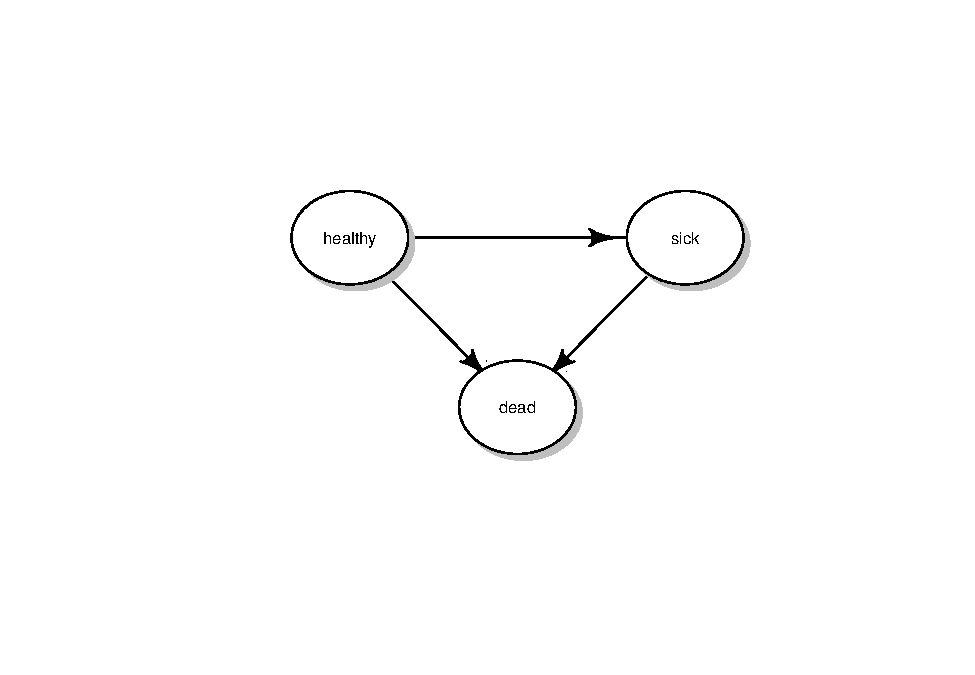
\includegraphics{markov_sick-sicker_solutions_files/figure-latex/unnamed-chunk-5-1.pdf}

\hypertarget{define-and-initialize-matrices-and-vectors}{%
\section{04 Define and initialize matrices and
vectors}\label{define-and-initialize-matrices-and-vectors}}

\hypertarget{cohort-trace}{%
\subsection{04.1 Cohort trace}\label{cohort-trace}}

\begin{Shaded}
\begin{Highlighting}[]
\CommentTok{# create the markov trace matrix M capturing the proportion of the cohort in each state }
\CommentTok{# at each cycle}
\NormalTok{m_M_notrt <-}\StringTok{ }\NormalTok{m_M_trt <-}\StringTok{ }\KeywordTok{matrix}\NormalTok{(}\OtherTok{NA}\NormalTok{, }
                               \DataTypeTok{nrow     =}\NormalTok{ n_t }\OperatorTok{+}\StringTok{ }\DecValTok{1}\NormalTok{, }\DataTypeTok{ncol =}\NormalTok{ n_states,}
                               \DataTypeTok{dimnames =} \KeywordTok{list}\NormalTok{(}\KeywordTok{paste}\NormalTok{(}\StringTok{"cycle"}\NormalTok{, }\DecValTok{0}\OperatorTok{:}\NormalTok{n_t, }\DataTypeTok{sep =} \StringTok{" "}\NormalTok{), v_n))}

\KeywordTok{head}\NormalTok{(m_M_notrt) }\CommentTok{# show first 6 rows of the matrix }
\end{Highlighting}
\end{Shaded}

\begin{verbatim}
##          H S1 S2  D
## cycle 0 NA NA NA NA
## cycle 1 NA NA NA NA
## cycle 2 NA NA NA NA
## cycle 3 NA NA NA NA
## cycle 4 NA NA NA NA
## cycle 5 NA NA NA NA
\end{verbatim}

\begin{Shaded}
\begin{Highlighting}[]
\CommentTok{# The cohort starts as healthy}
\NormalTok{m_M_notrt[}\DecValTok{1}\NormalTok{, ] <-}\StringTok{ }\NormalTok{m_M_trt[}\DecValTok{1}\NormalTok{, ] <-}\StringTok{ }\NormalTok{v_init  }\CommentTok{# initiate first cycle of cohort trace }
\end{Highlighting}
\end{Shaded}

\hypertarget{transition-probability-matrix}{%
\subsection{04.2 Transition probability
matrix}\label{transition-probability-matrix}}

\begin{Shaded}
\begin{Highlighting}[]
\CommentTok{# create the transition probability matrix for NO treatment}
\NormalTok{m_P_notrt <-}\StringTok{ }\NormalTok{m_P_trt  <-}\StringTok{ }\KeywordTok{matrix}\NormalTok{(}\DecValTok{0}\NormalTok{,}
                                \DataTypeTok{nrow =}\NormalTok{ n_states,}
                                \DataTypeTok{ncol =}\NormalTok{ n_states,}
                                \DataTypeTok{dimnames =} \KeywordTok{list}\NormalTok{(v_n, v_n)) }\CommentTok{# name the columns and rows of the matrix}
\NormalTok{m_P_notrt}
\end{Highlighting}
\end{Shaded}

\begin{verbatim}
##    H S1 S2 D
## H  0  0  0 0
## S1 0  0  0 0
## S2 0  0  0 0
## D  0  0  0 0
\end{verbatim}

\begin{Shaded}
\begin{Highlighting}[]
\NormalTok{m_P_trt}
\end{Highlighting}
\end{Shaded}

\begin{verbatim}
##    H S1 S2 D
## H  0  0  0 0
## S1 0  0  0 0
## S2 0  0  0 0
## D  0  0  0 0
\end{verbatim}

Fill in the transition probability matrix:

\begin{Shaded}
\begin{Highlighting}[]
\CommentTok{# from Healthy}
\NormalTok{m_P_notrt[}\StringTok{"H"}\NormalTok{, }\StringTok{"H"}\NormalTok{  ] <-}\StringTok{ }\NormalTok{(}\DecValTok{1} \OperatorTok{-}\StringTok{ }\NormalTok{p_HD) }\OperatorTok{*}\StringTok{ }\NormalTok{(}\DecValTok{1} \OperatorTok{-}\StringTok{ }\NormalTok{p_HS1)}
\NormalTok{m_P_notrt[}\StringTok{"H"}\NormalTok{, }\StringTok{"S1"}\NormalTok{ ] <-}\StringTok{ }\NormalTok{(}\DecValTok{1} \OperatorTok{-}\StringTok{ }\NormalTok{p_HD) }\OperatorTok{*}\StringTok{ }\NormalTok{p_HS1}
\NormalTok{m_P_notrt[}\StringTok{"H"}\NormalTok{, }\StringTok{"D"}\NormalTok{  ] <-}\StringTok{ }\NormalTok{p_HD}
\CommentTok{# from Sick}
\NormalTok{m_P_notrt[}\StringTok{"S1"}\NormalTok{, }\StringTok{"H"}\NormalTok{ ] <-}\StringTok{ }\NormalTok{(}\DecValTok{1} \OperatorTok{-}\StringTok{ }\NormalTok{p_S1D) }\OperatorTok{*}\StringTok{ }\NormalTok{p_S1H}
\NormalTok{m_P_notrt[}\StringTok{"S1"}\NormalTok{, }\StringTok{"S1"}\NormalTok{] <-}\StringTok{ }\NormalTok{(}\DecValTok{1} \OperatorTok{-}\StringTok{ }\NormalTok{p_S1D) }\OperatorTok{*}\StringTok{ }\NormalTok{(}\DecValTok{1} \OperatorTok{-}\StringTok{ }\NormalTok{(p_S1H }\OperatorTok{+}\StringTok{ }\NormalTok{p_S1S2))}
\NormalTok{m_P_notrt[}\StringTok{"S1"}\NormalTok{, }\StringTok{"S2"}\NormalTok{] <-}\StringTok{ }\NormalTok{(}\DecValTok{1} \OperatorTok{-}\StringTok{ }\NormalTok{p_S1D) }\OperatorTok{*}\StringTok{ }\NormalTok{p_S1S2}
\NormalTok{m_P_notrt[}\StringTok{"S1"}\NormalTok{, }\StringTok{"D"}\NormalTok{ ] <-}\StringTok{ }\NormalTok{p_S1D}
\CommentTok{# from Sicker}
\NormalTok{m_P_notrt[}\StringTok{"S2"}\NormalTok{, }\StringTok{"S2"}\NormalTok{] <-}\StringTok{ }\DecValTok{1} \OperatorTok{-}\StringTok{ }\NormalTok{p_S2D}
\NormalTok{m_P_notrt[}\StringTok{"S2"}\NormalTok{, }\StringTok{"D"}\NormalTok{ ] <-}\StringTok{ }\NormalTok{p_S2D}
\CommentTok{# from Dead}
\NormalTok{m_P_notrt[}\StringTok{"D"}\NormalTok{, }\StringTok{"D"}\NormalTok{  ] <-}\StringTok{ }\DecValTok{1}

\CommentTok{# Check that transition probabilities are in [0, 1]}
\KeywordTok{check_transition_probability}\NormalTok{(m_P_notrt, }\DataTypeTok{verbose =} \OtherTok{TRUE}\NormalTok{)}
\CommentTok{# Check that all rows sum to 1}
\KeywordTok{check_sum_of_transition_array}\NormalTok{(m_P_notrt, }\DataTypeTok{n_states =}\NormalTok{ n_states, }\DataTypeTok{n_cycles =}\NormalTok{ n_t, }\DataTypeTok{verbose =} \OtherTok{TRUE}\NormalTok{)}

\CommentTok{# create transition probability matrix for treatment same as no treatment}
\NormalTok{m_P_trt <-}\StringTok{ }\NormalTok{m_P_notrt}
\end{Highlighting}
\end{Shaded}

\hypertarget{run-markov-model}{%
\section{05 Run Markov model}\label{run-markov-model}}

\begin{Shaded}
\begin{Highlighting}[]
\ControlFlowTok{for}\NormalTok{ (t }\ControlFlowTok{in} \DecValTok{1}\OperatorTok{:}\NormalTok{n_t)\{  }\CommentTok{# loop through the number of cycles}
\NormalTok{  m_M_notrt[t }\OperatorTok{+}\StringTok{ }\DecValTok{1}\NormalTok{, ] <-}\StringTok{ }\KeywordTok{t}\NormalTok{(m_M_notrt[t, ]) }\OperatorTok\StringTok{ }\NormalTok{m_P_notrt  }\CommentTok{# estimate the Markov trace }
                                                         \CommentTok{# for the next cycle (t + 1)}
\NormalTok{  m_M_trt[t }\OperatorTok{+}\StringTok{ }\DecValTok{1}\NormalTok{, ]   <-}\StringTok{ }\KeywordTok{t}\NormalTok{(m_M_trt[t, ])   }\OperatorTok\StringTok{ }\NormalTok{m_P_trt    }\CommentTok{# estimate the Markov trace }
                                                         \CommentTok{# for the next cycle (t + 1)}
\NormalTok{\} }\CommentTok{# close the loop}

\KeywordTok{head}\NormalTok{(m_M_notrt)  }\CommentTok{# show the first 6 lines of the matrix}
\end{Highlighting}
\end{Shaded}

\begin{verbatim}
##                 H        S1         S2          D
## cycle 0 1.0000000 0.0000000 0.00000000 0.00000000
## cycle 1 0.8457500 0.1492500 0.00000000 0.00500000
## cycle 2 0.7888043 0.1843020 0.01543735 0.01145632
## cycle 3 0.7579069 0.1894418 0.03374551 0.01890581
## cycle 4 0.7343069 0.1868303 0.05169021 0.02717260
## cycle 5 0.7130610 0.1822918 0.06848747 0.03615973
\end{verbatim}

\hypertarget{compute-and-plot-epidemiological-outcomes}{%
\section{06 Compute and Plot Epidemiological
Outcomes}\label{compute-and-plot-epidemiological-outcomes}}

\hypertarget{cohort-trace-1}{%
\subsection{06.1 Cohort trace}\label{cohort-trace-1}}

The transition probabilities are similari in both strategies. Therefore,
the cohort trace figure applies to both strategies.

\begin{Shaded}
\begin{Highlighting}[]
\CommentTok{# create a plot of the data}
\KeywordTok{matplot}\NormalTok{(m_M_notrt, }\DataTypeTok{type =} \StringTok{'l'}\NormalTok{, }
        \DataTypeTok{ylab =} \StringTok{"Probability of state occupancy"}\NormalTok{,}
        \DataTypeTok{xlab =} \StringTok{"Cycle"}\NormalTok{,}
        \DataTypeTok{main =} \StringTok{"Cohort Trace "}\NormalTok{)             }
\CommentTok{# add a legend to the graph}
\KeywordTok{legend}\NormalTok{(}\StringTok{"topright"}\NormalTok{, v_n, }\DataTypeTok{col =} \DecValTok{1}\OperatorTok{:}\NormalTok{n_states, }\DataTypeTok{lty =} \DecValTok{1}\OperatorTok{:}\NormalTok{n_states, }\DataTypeTok{bty =} \StringTok{"n"}\NormalTok{) }
\end{Highlighting}
\end{Shaded}

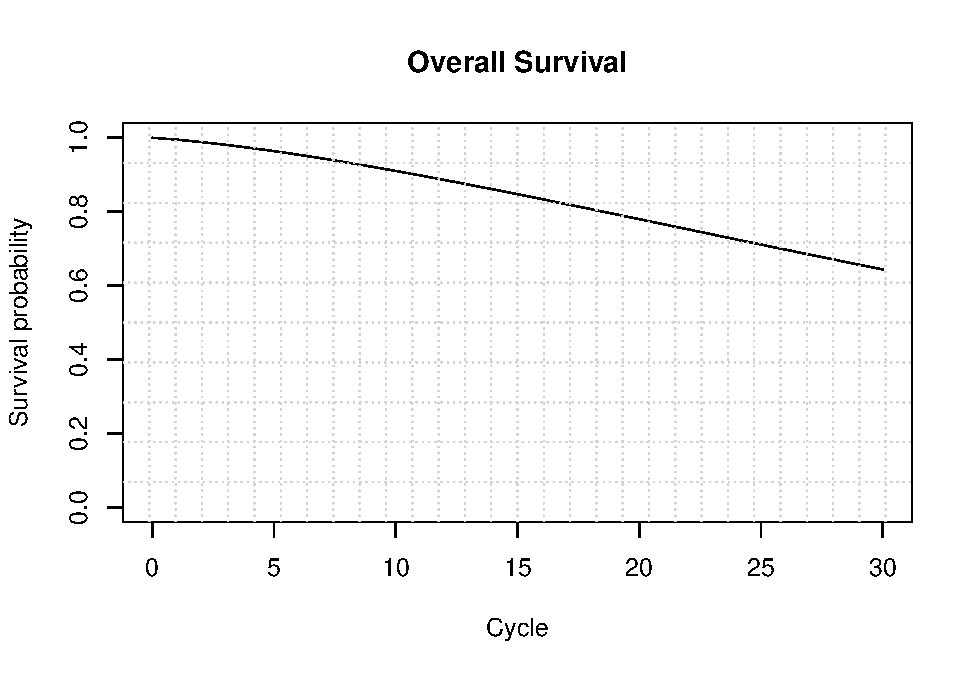
\includegraphics{markov_sick-sicker_solutions_files/figure-latex/unnamed-chunk-10-1.pdf}

\hypertarget{overall-survival-os}{%
\subsection{06.2 Overall Survival (OS)}\label{overall-survival-os}}

\begin{Shaded}
\begin{Highlighting}[]
\CommentTok{# calculate the overall survival (OS) probability for no treatment}
\NormalTok{v_os_notrt <-}\StringTok{ }\DecValTok{1} \OperatorTok{-}\StringTok{ }\NormalTok{m_M_notrt[, }\StringTok{"D"}\NormalTok{]    }
\CommentTok{# alternative way of calculating the OS probability   }
\NormalTok{v_os_notrt <-}\StringTok{ }\KeywordTok{rowSums}\NormalTok{(m_M_notrt[, }\DecValTok{1}\OperatorTok{:}\DecValTok{3}\NormalTok{])  }
\CommentTok{# create a simple plot showing the OS}
\KeywordTok{plot}\NormalTok{(}\DecValTok{0}\OperatorTok{:}\NormalTok{n_t, v_os_notrt, }\DataTypeTok{type =} \StringTok{'l'}\NormalTok{, }
     \DataTypeTok{ylim =} \KeywordTok{c}\NormalTok{(}\DecValTok{0}\NormalTok{, }\DecValTok{1}\NormalTok{),}
     \DataTypeTok{ylab =} \StringTok{"Survival probability"}\NormalTok{,}
     \DataTypeTok{xlab =} \StringTok{"Cycle"}\NormalTok{,}
     \DataTypeTok{main =} \StringTok{"Overall Survival"}\NormalTok{)          }
\CommentTok{# add grid }
\KeywordTok{grid}\NormalTok{(}\DataTypeTok{nx =}\NormalTok{ n_t, }\DataTypeTok{ny =} \DecValTok{10}\NormalTok{, }\DataTypeTok{col =} \StringTok{"lightgray"}\NormalTok{, }\DataTypeTok{lty =} \StringTok{"dotted"}\NormalTok{, }\DataTypeTok{lwd =} \KeywordTok{par}\NormalTok{(}\StringTok{"lwd"}\NormalTok{), }
     \DataTypeTok{equilogs =} \OtherTok{TRUE}\NormalTok{) }
\end{Highlighting}
\end{Shaded}

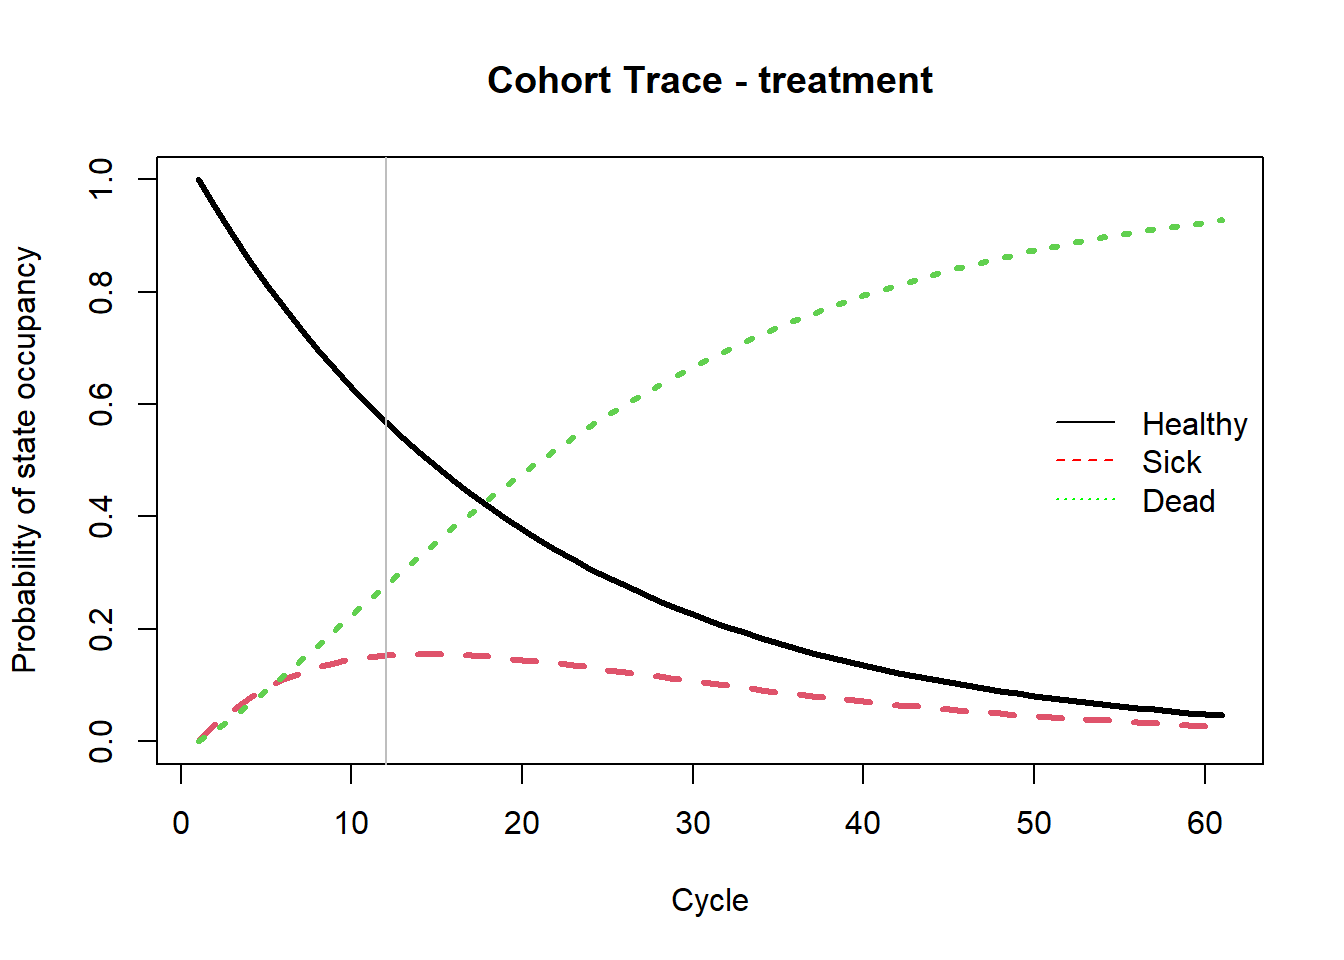
\includegraphics{markov_sick-sicker_solutions_files/figure-latex/unnamed-chunk-11-1.pdf}

\hypertarget{life-expectancy-le}{%
\subsection{06.2.1 Life Expectancy (LE)}\label{life-expectancy-le}}

\begin{Shaded}
\begin{Highlighting}[]
\NormalTok{v_le <-}\StringTok{ }\KeywordTok{sum}\NormalTok{(v_os_notrt)  }\CommentTok{# summing probability of OS over time  (i.e. life expectancy)}
\end{Highlighting}
\end{Shaded}

\hypertarget{disease-prevalence}{%
\subsection{06.3 Disease prevalence}\label{disease-prevalence}}

\begin{Shaded}
\begin{Highlighting}[]
\NormalTok{v_prev <-}\StringTok{ }\KeywordTok{rowSums}\NormalTok{(m_M_notrt[, }\KeywordTok{c}\NormalTok{(}\StringTok{"S1"}\NormalTok{, }\StringTok{"S2"}\NormalTok{)]) }\OperatorTok{/}\StringTok{ }\NormalTok{v_os_notrt}
\KeywordTok{plot}\NormalTok{(v_prev,}
     \DataTypeTok{ylim =} \KeywordTok{c}\NormalTok{(}\DecValTok{0}\NormalTok{, }\DecValTok{1}\NormalTok{),}
     \DataTypeTok{ylab =} \StringTok{"Prevalence"}\NormalTok{,}
     \DataTypeTok{xlab =} \StringTok{"Cycle"}\NormalTok{,}
     \DataTypeTok{main =} \StringTok{"Disease prevalence"}\NormalTok{)}
\end{Highlighting}
\end{Shaded}

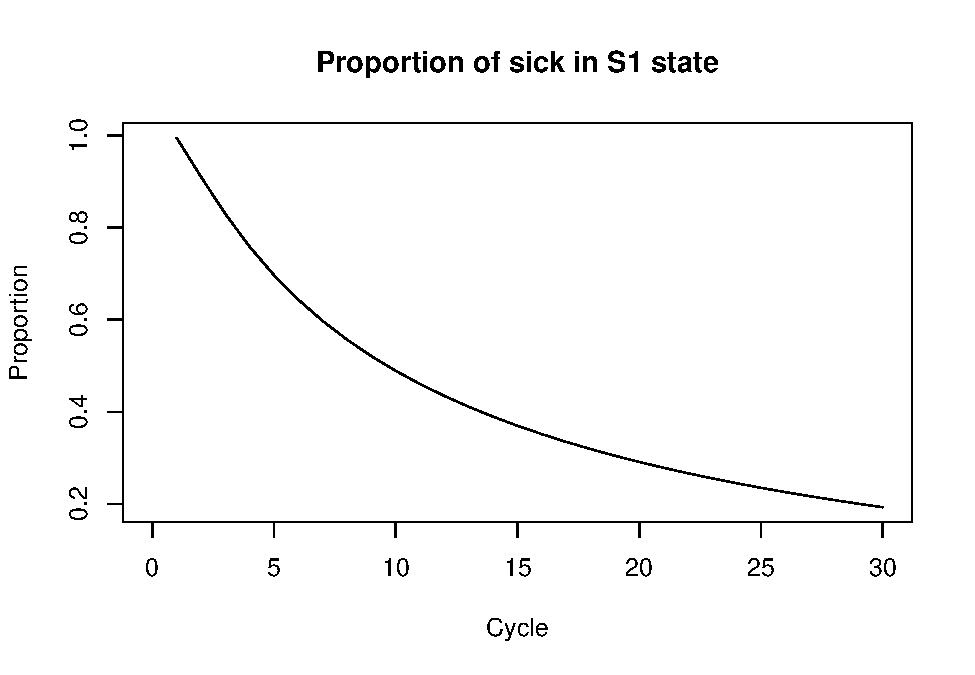
\includegraphics{markov_sick-sicker_solutions_files/figure-latex/unnamed-chunk-13-1.pdf}

\hypertarget{proportion-of-sick-in-s1-state}{%
\subsection{06.4 Proportion of sick in S1
state}\label{proportion-of-sick-in-s1-state}}

\begin{Shaded}
\begin{Highlighting}[]
\NormalTok{v_prop_S1 <-}\StringTok{ }\NormalTok{m_M_notrt[, }\StringTok{"S1"}\NormalTok{] }\OperatorTok{/}\StringTok{ }\NormalTok{v_prev}
\KeywordTok{plot}\NormalTok{(}\DecValTok{0}\OperatorTok{:}\NormalTok{n_t, v_prop_S1,}
     \DataTypeTok{xlab =} \StringTok{"Cycle"}\NormalTok{, }
     \DataTypeTok{ylab =} \StringTok{"Proportion"}\NormalTok{, }
     \DataTypeTok{main =} \StringTok{"Proportion of sick in S1 state"}\NormalTok{, }
     \DataTypeTok{col  =} \StringTok{"black"}\NormalTok{, }\DataTypeTok{type =} \StringTok{"l"}\NormalTok{)}
\end{Highlighting}
\end{Shaded}

\includegraphics{markov_sick-sicker_solutions_files/figure-latex/unnamed-chunk-14-1.pdf}

\hypertarget{compute-cost-effectiveness-outcomes}{%
\section{07 Compute Cost-Effectiveness
Outcomes}\label{compute-cost-effectiveness-outcomes}}

\begin{Shaded}
\begin{Highlighting}[]
\CommentTok{# Vectors with costs and utilities by treatment}
\NormalTok{v_u_notrt   <-}\StringTok{ }\KeywordTok{c}\NormalTok{(u_H, u_S1,  u_S2, u_D)}
\NormalTok{v_u_trt     <-}\StringTok{ }\KeywordTok{c}\NormalTok{(u_H, u_trt, u_S2, u_D)}

\NormalTok{v_c_notrt   <-}\StringTok{ }\KeywordTok{c}\NormalTok{(c_H, c_S1,         c_S2,         c_D)}
\NormalTok{v_c_trt     <-}\StringTok{ }\KeywordTok{c}\NormalTok{(c_H, c_S1 }\OperatorTok{+}\StringTok{ }\NormalTok{c_trt, c_S2 }\OperatorTok{+}\StringTok{ }\NormalTok{c_trt, c_D)}
\end{Highlighting}
\end{Shaded}

\hypertarget{mean-costs-and-qalys-for-treatment-and-no-treatment}{%
\subsection{07.1 Mean Costs and QALYs for Treatment and NO
Treatment}\label{mean-costs-and-qalys-for-treatment-and-no-treatment}}

\begin{Shaded}
\begin{Highlighting}[]
\NormalTok{v_tu_notrt  <-}\StringTok{ }\NormalTok{m_M_notrt   }\OperatorTok\StringTok{  }\NormalTok{v_u_notrt}
\NormalTok{v_tu_trt    <-}\StringTok{ }\NormalTok{m_M_trt     }\OperatorTok\StringTok{  }\NormalTok{v_u_trt}

\NormalTok{v_tc_notrt  <-}\StringTok{ }\NormalTok{m_M_notrt   }\OperatorTok\StringTok{  }\NormalTok{v_c_notrt}
\NormalTok{v_tc_trt    <-}\StringTok{ }\NormalTok{m_M_trt     }\OperatorTok\StringTok{  }\NormalTok{v_c_trt }
\end{Highlighting}
\end{Shaded}

\hypertarget{discounted-mean-costs-and-qalys}{%
\subsection{07.2 Discounted Mean Costs and
QALYs}\label{discounted-mean-costs-and-qalys}}

\begin{Shaded}
\begin{Highlighting}[]
\NormalTok{tu_d_notrt  <-}\StringTok{ }\KeywordTok{t}\NormalTok{(v_tu_notrt)   }\OperatorTok\StringTok{  }\NormalTok{v_dwe   }
\NormalTok{tu_d_trt    <-}\StringTok{ }\KeywordTok{t}\NormalTok{(v_tu_trt)     }\OperatorTok\StringTok{  }\NormalTok{v_dwe}

\NormalTok{tc_d_notrt  <-}\StringTok{ }\KeywordTok{t}\NormalTok{(v_tc_notrt)   }\OperatorTok\StringTok{  }\NormalTok{v_dwc}
\NormalTok{tc_d_trt    <-}\StringTok{ }\KeywordTok{t}\NormalTok{(v_tc_trt)     }\OperatorTok\StringTok{  }\NormalTok{v_dwc}

\CommentTok{# store them into a vector}
\NormalTok{v_tc_d      <-}\StringTok{ }\KeywordTok{c}\NormalTok{(tc_d_notrt, tc_d_trt)}
\NormalTok{v_tu_d      <-}\StringTok{ }\KeywordTok{c}\NormalTok{(tu_d_notrt, tu_d_trt)}

\CommentTok{# Dataframe with discounted costs and effectiveness}
\NormalTok{df_ce       <-}\StringTok{ }\KeywordTok{data.frame}\NormalTok{(}\DataTypeTok{Strategy =}\NormalTok{ v_names_str,}
                          \DataTypeTok{Cost     =}\NormalTok{ v_tc_d,}
                          \DataTypeTok{Effect   =}\NormalTok{ v_tu_d}
\NormalTok{                          )}
\NormalTok{df_ce}
\end{Highlighting}
\end{Shaded}

\begin{verbatim}
##       Strategy      Cost   Effect
## 1 No Treatment  75795.04 15.84802
## 2    Treatment 141511.41 16.41446
\end{verbatim}

\hypertarget{compute-icers-of-the-markov-model}{%
\subsection{07.3 Compute ICERs of the Markov
model}\label{compute-icers-of-the-markov-model}}

\begin{Shaded}
\begin{Highlighting}[]
\NormalTok{df_cea <-}\StringTok{ }\KeywordTok{calculate_icers}\NormalTok{(}\DataTypeTok{cost       =}\NormalTok{ df_ce}\OperatorTok{$}\NormalTok{Cost,}
                          \DataTypeTok{effect     =}\NormalTok{ df_ce}\OperatorTok{$}\NormalTok{Effect,}
                          \DataTypeTok{strategies =}\NormalTok{ df_ce}\OperatorTok{$}\NormalTok{Strategy}
\NormalTok{                          )}
\NormalTok{df_cea}
\end{Highlighting}
\end{Shaded}

\begin{verbatim}
##       Strategy      Cost   Effect Inc_Cost Inc_Effect     ICER Status
## 1 No Treatment  75795.04 15.84802       NA         NA       NA     ND
## 2    Treatment 141511.41 16.41446 65716.37  0.5664367 116017.2     ND
\end{verbatim}

\hypertarget{plot-frontier-of-the-markov-model}{%
\subsection{07.4 Plot frontier of the Markov
model}\label{plot-frontier-of-the-markov-model}}

\begin{Shaded}
\begin{Highlighting}[]
\KeywordTok{plot}\NormalTok{(df_cea, }\DataTypeTok{effect_units =} \StringTok{"QALYs"}\NormalTok{, }\DataTypeTok{xlim =} \KeywordTok{c}\NormalTok{(}\FloatTok{15.6}\NormalTok{, }\FloatTok{16.6}\NormalTok{))}
\end{Highlighting}
\end{Shaded}

\includegraphics{markov_sick-sicker_solutions_files/figure-latex/unnamed-chunk-19-1.pdf}

\end{document}
